% =====================================================================
%  Aprendizaje No Supervisado — Sesión 3: Agrupamiento jerárquico
%  Unidad 1: Algoritmos de agrupamiento
%  Compilar con: latexmk -pdf Sesion3-Jerarquico.tex
%  Figuras: python3 figuras/generar_figuras.py
%  El laboratorio está en Laboratorio.tex (se incluye al final con \input)
% =====================================================================
\documentclass[aspectratio=169,11pt]{beamer}

\usepackage[utf8]{inputenc}
\usepackage[T1]{fontenc}
\usepackage[spanish,es-noshorthands,es-nodecimaldot]{babel}
\usepackage{amsmath,amssymb,bm}
\usepackage{booktabs,array}
\usepackage{listings}
\usepackage{tikz}
\usetikzlibrary{positioning,arrows.meta}
\graphicspath{{figuras/}}
\tikzset{caja/.style={draw=azul,fill=azul!10,rounded corners,align=center,font=\small,
  minimum height=9mm}}

% ---------- Tema (común a las presentaciones del curso) ----------
\usetheme{Madrid}
\usefonttheme{professionalfonts}
\definecolor{marino}{HTML}{1F3864}
\definecolor{azul}{HTML}{2E75B6}
\definecolor{naranja}{HTML}{E07B22}
\definecolor{verde}{HTML}{5B9A3C}
\definecolor{fondocod}{HTML}{F4F6F9}
\setbeamercolor{palette primary}{bg=marino,fg=white}
\setbeamercolor{palette secondary}{bg=azul,fg=white}
\setbeamercolor{palette tertiary}{bg=marino,fg=white}
\setbeamercolor{frametitle}{bg=marino,fg=white}
\setbeamercolor{title}{bg=marino,fg=white}
\setbeamercolor{structure}{fg=azul}
\setbeamercolor{block title}{bg=azul,fg=white}
\setbeamercolor{block body}{bg=azul!8}
\setbeamercolor{block title alerted}{bg=naranja,fg=white}
\setbeamercolor{block body alerted}{bg=naranja!10}
\setbeamercolor{block title example}{bg=verde,fg=white}
\setbeamercolor{block body example}{bg=verde!10}
\setbeamercolor{alerted text}{fg=naranja}
\setbeamertemplate{navigation symbols}{}
\setbeamertemplate{itemize items}[circle]
\setbeamertemplate{blocks}[rounded][shadow=false]

\AtBeginSection[]{
  \begin{frame}
    \vfill\centering
    \begin{beamercolorbox}[sep=12pt,center,rounded=true]{title}
      \usebeamerfont{title}\insertsectionhead
    \end{beamercolorbox}
    \vfill
  \end{frame}
}

\lstdefinestyle{py}{
  language=Python, basicstyle=\ttfamily\scriptsize,
  keywordstyle=\color{marino}\bfseries, commentstyle=\color{gray}\itshape,
  stringstyle=\color{naranja}, backgroundcolor=\color{fondocod},
  frame=single, rulecolor=\color{azul!40}, showstringspaces=false,
  columns=fullflexible, breaklines=true, xleftmargin=4pt, xrightmargin=4pt
}
\lstset{style=py}

\newcommand{\R}{\mathbb{R}}
\newcommand{\x}{\bm{x}}
\newcommand{\muv}{\bm{\mu}}

\title[Sesión 3: Agrupamiento jerárquico]{Sesión 3: Agrupamiento jerárquico}
\subtitle{Aprendizaje No Supervisado --- Unidad 1: Algoritmos de agrupamiento}
\author[A. Espinosa Romero]{Arturo Espinosa Romero}
\institute[FMAT]{Maestría en Inteligencia Artificial \\ Facultad de Matemáticas}
\date{Sesión 3}

% =====================================================================
\begin{document}

\begin{frame}
  \titlepage
\end{frame}

\begin{frame}{Agenda de la sesión}
  \begin{columns}[T]
    \column{0.55\textwidth}
    \begin{enumerate}
      \item Grupos anidados: la idea jerárquica
      \item Enfoques aglomerativo y divisivo
      \item Criterios de enlace: simple, completo, promedio y Ward
      \item Dendrogramas y corte del árbol
      \item Complejidad computacional y escalabilidad
      \item Laboratorio: agrupamiento jerárquico de Iris con SciPy
    \end{enumerate}
    \column{0.4\textwidth}
    \begin{block}{Al terminar podrás}
      \begin{itemize}
        \item Explicar cómo se construye una jerarquía de grupos
        \item Elegir un criterio de enlace según la forma de los grupos
        \item Leer y cortar un dendrograma
        \item Saber cuándo el método no escala
      \end{itemize}
    \end{block}
  \end{columns}
\end{frame}

% =====================================================================
\section{Grupos anidados}
% =====================================================================

\begin{frame}{Problema detonador: ¿y si no queremos fijar $k$?}
  \centering
  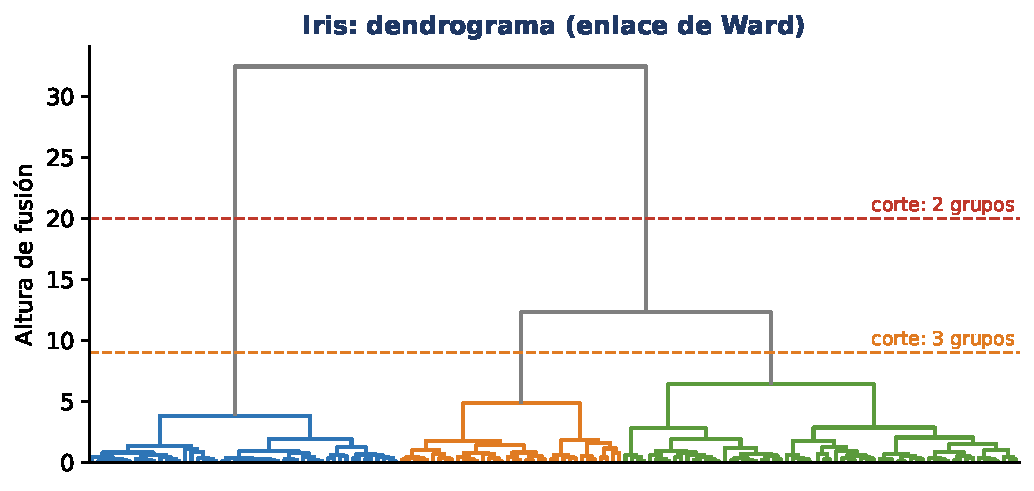
\includegraphics[width=0.8\textwidth]{iris_dendrograma}
  \begin{itemize}
    \item En la Sesión 2 elegimos $k=3$ para Iris; el método de silueta favorecía $k=2$.
    \item Ambas respuestas tienen sentido: setosa se separa primero, y después
          versicolor y virginica.
    \item Un \alert{dendrograma} muestra la estructura a todas las escalas a la vez,
          sin fijar $k$ de antemano.
  \end{itemize}
\end{frame}

\begin{frame}{Una jerarquía de particiones}
  El agrupamiento jerárquico produce una sucesión de particiones \alert{anidadas}:
  \[
    \mathcal{P}_n \;\prec\; \mathcal{P}_{n-1} \;\prec\; \cdots \;\prec\; \mathcal{P}_2 \;\prec\; \mathcal{P}_1 ,
  \]
  donde $\mathcal{P}_n$ tiene un grupo por punto, $\mathcal{P}_1$ un solo grupo, y cada
  $\mathcal{P}_{k}$ se obtiene uniendo dos grupos de $\mathcal{P}_{k+1}$.
  \vspace{6pt}
  \begin{columns}[T]
    \column{0.48\textwidth}
    \begin{block}{Ventajas}
      \begin{itemize}
        \item No hay que fijar $k$: se elige al final.
        \item Es determinista: no depende de una inicialización.
        \item El dendrograma es interpretable.
      \end{itemize}
    \end{block}
    \column{0.48\textwidth}
    \begin{alertblock}{Costos}
      \begin{itemize}
        \item Una fusión nunca se deshace (algoritmo voraz).
        \item Requiere todas las distancias: memoria $O(n^2)$.
        \item El resultado depende del criterio de enlace.
      \end{itemize}
    \end{alertblock}
  \end{columns}
\end{frame}

% =====================================================================
\section{Enfoques aglomerativo y divisivo}
% =====================================================================

\begin{frame}{Dos maneras de construir el árbol}
  \centering
  \begin{tikzpicture}[node distance=5mm and 10mm]
    \node[caja] (n) {$n$ grupos\\(cada punto solo)};
    \node[caja,right=25mm of n] (m) {particiones\\intermedias};
    \node[caja,right=25mm of m] (u) {1 grupo\\(todos los puntos)};
    \draw[-{Stealth},thick,azul] ([yshift=3mm]n.east) -- node[above,font=\small]{aglomerativo: unir} ([yshift=3mm]m.west);
    \draw[-{Stealth},thick,azul] ([yshift=3mm]m.east) -- node[above,font=\small]{unir} ([yshift=3mm]u.west);
    \draw[-{Stealth},thick,naranja] ([yshift=-3mm]u.west) -- node[below,font=\small]{dividir} ([yshift=-3mm]m.east);
    \draw[-{Stealth},thick,naranja] ([yshift=-3mm]m.west) -- node[below,font=\small]{divisivo: dividir} ([yshift=-3mm]n.east);
  \end{tikzpicture}
  \vspace{8pt}
  \begin{columns}[T]
    \column{0.48\textwidth}
    \begin{block}{Aglomerativo (de abajo hacia arriba)}
      Empieza con $n$ grupos de un punto y une, en cada paso, los dos grupos más cercanos.
      Es el más usado.
    \end{block}
    \column{0.48\textwidth}
    \begin{block}{Divisivo (de arriba hacia abajo)}
      Empieza con un grupo y divide, en cada paso, el grupo menos homogéneo.
    \end{block}
  \end{columns}
\end{frame}

\begin{frame}{Algoritmo aglomerativo}
  \begin{enumerate}
    \item Calcular la matriz de distancias $d(\x_i,\x_j)$ entre todos los pares de puntos.
    \item Iniciar con $n$ grupos: $\{\x_1\},\dots,\{\x_n\}$.
    \item Repetir $n-1$ veces:
      \begin{enumerate}
        \item Encontrar los dos grupos $A$ y $B$ con menor distancia $D(A,B)$.
        \item Unirlos en $A\cup B$ y registrar la \textbf{altura} de la fusión, $D(A,B)$.
        \item Actualizar las distancias entre $A\cup B$ y los demás grupos.
      \end{enumerate}
  \end{enumerate}
  \vspace{6pt}
  \begin{alertblock}{La decisión clave}
    Cómo medir la distancia $D(A,B)$ \textbf{entre grupos} a partir de las distancias entre
    puntos: el \textbf{criterio de enlace} (\emph{linkage}).
  \end{alertblock}
\end{frame}

\begin{frame}{Enfoque divisivo}
  \begin{itemize}
    \item Un grupo con $m$ puntos se puede partir en dos de $2^{m-1}-1$ maneras:
          no se pueden revisar todas. Se usan heurísticas.
    \item \textbf{DIANA} (Kaufman y Rousseeuw, 1990): en el grupo más disperso, el punto con
          mayor distancia media a los demás inicia un grupo ``disidente'', que va atrayendo
          a los puntos más cercanos a él que al resto.
    \item \textbf{k-medias bisectante}: dividir con k-medias de $k=2$ el grupo con mayor inercia,
          y repetir (\texttt{sklearn.cluster.BisectingKMeans}).
  \end{itemize}
  \vspace{6pt}
  \begin{block}{Cuándo considerarlo}
    Cuando interesan las primeras divisiones (pocos grupos grandes): el divisivo las decide
    con toda la información, mientras que el aglomerativo llega a ellas al final, después de
    muchas fusiones locales.
  \end{block}
\end{frame}

% =====================================================================
\section{Criterios de enlace}
% =====================================================================

\begin{frame}{Cuatro criterios de enlace}
  Distancia entre los grupos $A$ y $B$:
  \renewcommand{\arraystretch}{1.6}
  \begin{tabular}{@{}lll@{}}
    \toprule
    \textbf{Enlace} & \textbf{Definición} & \textbf{Comportamiento}\\
    \midrule
    Simple   & $\displaystyle\min_{a\in A,\,b\in B} d(a,b)$ & Formas alargadas; efecto \alert{cadena} \\
    Completo & $\displaystyle\max_{a\in A,\,b\in B} d(a,b)$ & Grupos compactos; sensible a atípicos \\
    Promedio & $\displaystyle\frac{1}{|A||B|}\sum_{a\in A}\sum_{b\in B} d(a,b)$ & Intermedio \\
    Ward     & $\displaystyle\frac{|A||B|}{|A|+|B|}\lVert\muv_A-\muv_B\rVert^2$ & Aumento mínimo de la inercia \\
    \bottomrule
  \end{tabular}
  \vspace{4pt}\\
  {\small Simple, completo y promedio admiten cualquier disimilitud. Ward requiere distancia euclidiana.}
\end{frame}

\begin{frame}{Ejemplo: el mismo dato, tres árboles}
  Puntos en una dimensión: $x=\{1,\ 2,\ 4,\ 7,\ 11\}$.
  \vspace{2pt}
  \begin{center}
    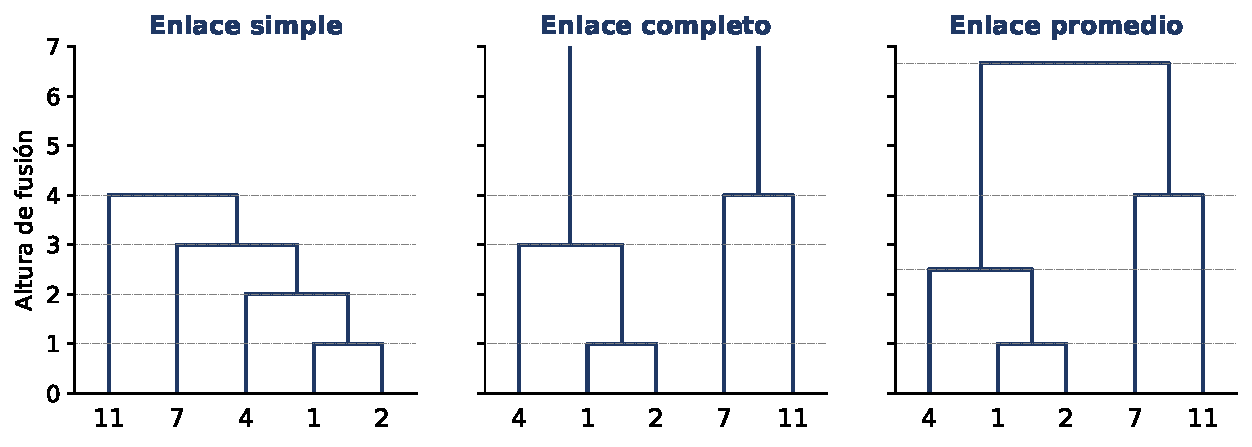
\includegraphics[width=0.66\textwidth]{ejemplo_1d}
  \end{center}
  \vspace{-6pt}
  \footnotesize
  \begin{tabular}{@{}llll@{}}
    \toprule
    \textbf{Fusión} & \textbf{Simple} & \textbf{Completo} & \textbf{Promedio}\\
    \midrule
    1.ª & $\{1,2\}$ a 1 & $\{1,2\}$ a 1 & $\{1,2\}$ a 1 \\
    2.ª & $\{1,2,4\}$ a 2 & $\{1,2,4\}$ a 3 & $\{1,2,4\}$ a 2.5 \\
    3.ª & $\{1,2,4,7\}$ a 3 & $\{7,11\}$ a 4 & $\{7,11\}$ a 4 \\
    4.ª & todos a 4 & todos a 10 & todos a 6.67 \\
    \bottomrule
  \end{tabular}
  \quad
  \begin{minipage}[m]{0.33\textwidth}
    El enlace simple agrega los puntos de uno en uno (cadena); el completo y el promedio
    forman dos grupos: $\{1,2,4\}$ y $\{7,11\}$.
  \end{minipage}
\end{frame}

\begin{frame}{Actualización de distancias: fórmula de Lance y Williams}
  Al unir $A$ y $B$, la distancia del nuevo grupo a otro grupo $C$ se calcula sin volver a los puntos:
  \[
    D(C, A\cup B) = \alpha_A D(C,A) + \alpha_B D(C,B) + \beta\, D(A,B) + \gamma\,\lvert D(C,A)-D(C,B)\rvert .
  \]
  \renewcommand{\arraystretch}{1.5}
  \centering
  \begin{tabular}{@{}lcccc@{}}
    \toprule
    \textbf{Enlace} & $\alpha_A$ & $\alpha_B$ & $\beta$ & $\gamma$\\
    \midrule
    Simple   & $\tfrac12$ & $\tfrac12$ & 0 & $-\tfrac12$ \\
    Completo & $\tfrac12$ & $\tfrac12$ & 0 & $\tfrac12$ \\
    Promedio & $\tfrac{n_A}{n_A+n_B}$ & $\tfrac{n_B}{n_A+n_B}$ & 0 & 0 \\
    Ward (distancias al cuadrado) & $\tfrac{n_A+n_C}{n_A+n_B+n_C}$ & $\tfrac{n_B+n_C}{n_A+n_B+n_C}$ & $\tfrac{-n_C}{n_A+n_B+n_C}$ & 0 \\
    \bottomrule
  \end{tabular}\\[6pt]
  \raggedright
  {\small Así cada fusión sólo actualiza una fila de la matriz de distancias.}
\end{frame}

\begin{frame}{El enlace de Ward}
  \begin{itemize}
    \item Une los dos grupos cuya fusión \alert{aumenta menos la inercia}
          $J=\sum_j\sum_{i\in C_j}\lVert\x_i-\muv_j\rVert^2$ de la Sesión 2:
          \[
            \Delta J(A,B) = \frac{|A||B|}{|A|+|B|}\,\lVert\muv_A-\muv_B\rVert^2 .
          \]
    \item Es una versión \textbf{voraz} del objetivo de k-medias: por eso produce grupos
          compactos y de tamaño parecido, y resultados similares a k-medias.
    \item A diferencia de k-medias, no reasigna puntos: una fusión no se deshace.
    \item En SciPy la altura de la fusión es $\sqrt{2\,\Delta J}$; con dos puntos
          coincide con su distancia euclidiana.
  \end{itemize}
\end{frame}

\begin{frame}{Enlace simple y árbol de expansión mínima}
  \begin{columns}[c]
    \column{0.45\textwidth}
    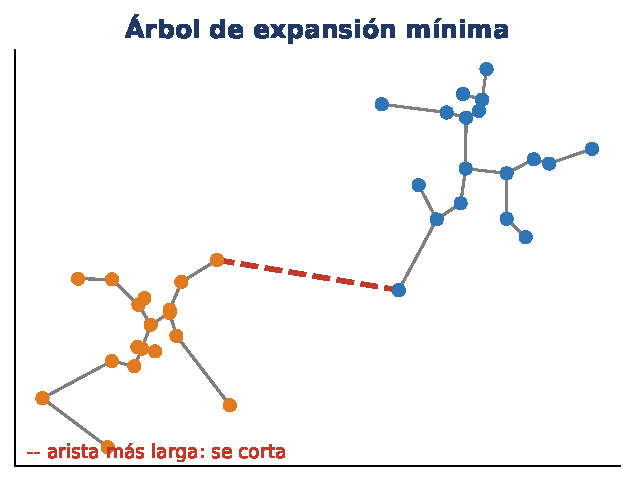
\includegraphics[width=\textwidth]{arbol_minimo}
    \column{0.52\textwidth}
    \begin{itemize}
      \item El enlace simple equivale a construir el \textbf{árbol de expansión mínima}
            de los puntos y cortar sus $k-1$ aristas más largas (Gower y Ross, 1969).
      \item Por eso sigue estructuras alargadas y no convexas.
      \item Y por eso basta una ``hilera'' de puntos intermedios para unir dos grupos
            distintos: el \alert{efecto cadena}.
    \end{itemize}
  \end{columns}
\end{frame}

\begin{frame}{El efecto del enlace}
  \centering
  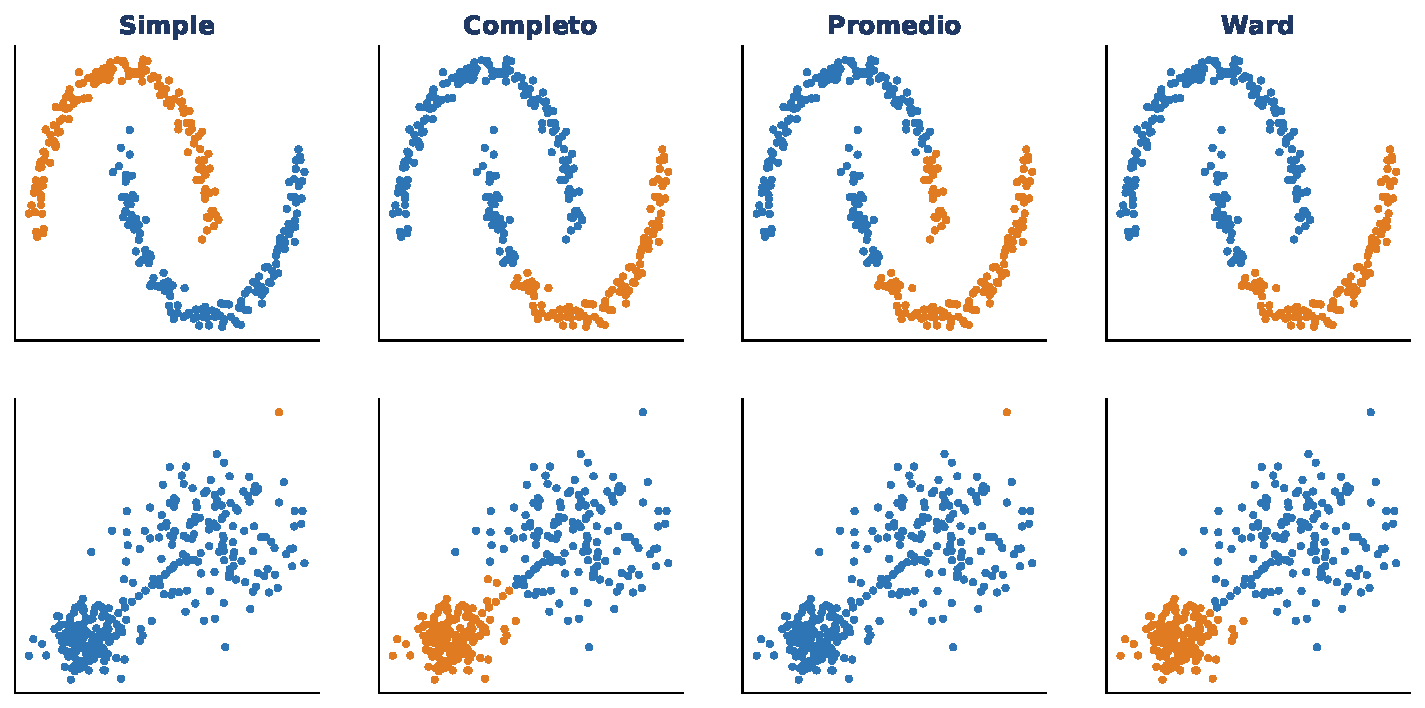
\includegraphics[width=0.82\textwidth]{enlaces}
  \begin{itemize}
    \item Arriba: el enlace simple recupera las lunas; completo, promedio y Ward las cortan.
    \item Abajo: un puente de 12 puntos basta para que el enlace simple encadene los dos grupos.
  \end{itemize}
\end{frame}

\begin{frame}{Otros enlaces y sus riesgos}
  \begin{itemize}
    \item \textbf{Centroide}: distancia entre las medias de los grupos.
    \item \textbf{Mediana} (o WPGMC): como el centroide, pero sin ponderar por el tamaño.
  \end{itemize}
  \begin{alertblock}{Inversiones}
    Con centroide y mediana una fusión posterior puede ocurrir a \emph{menor} altura que una
    anterior: el dendrograma deja de ser monótono y no se puede cortar por altura.
    Simple, completo, promedio y Ward nunca producen inversiones.
  \end{alertblock}
  \vspace{4pt}
  \begin{block}{Guía rápida}
    \begin{itemize}
      \item Grupos compactos y de tamaño parecido: \textbf{Ward}.
      \item Sin suposición de forma, buen compromiso general: \textbf{promedio}.
      \item Formas alargadas bien separadas y sin ruido: \textbf{simple}.
      \item Disimilitudes no euclidianas: promedio o completo, no Ward.
    \end{itemize}
  \end{block}
\end{frame}

% =====================================================================
\section{Dendrogramas y corte del árbol}
% =====================================================================

\begin{frame}{Cómo leer un dendrograma}
  \centering
  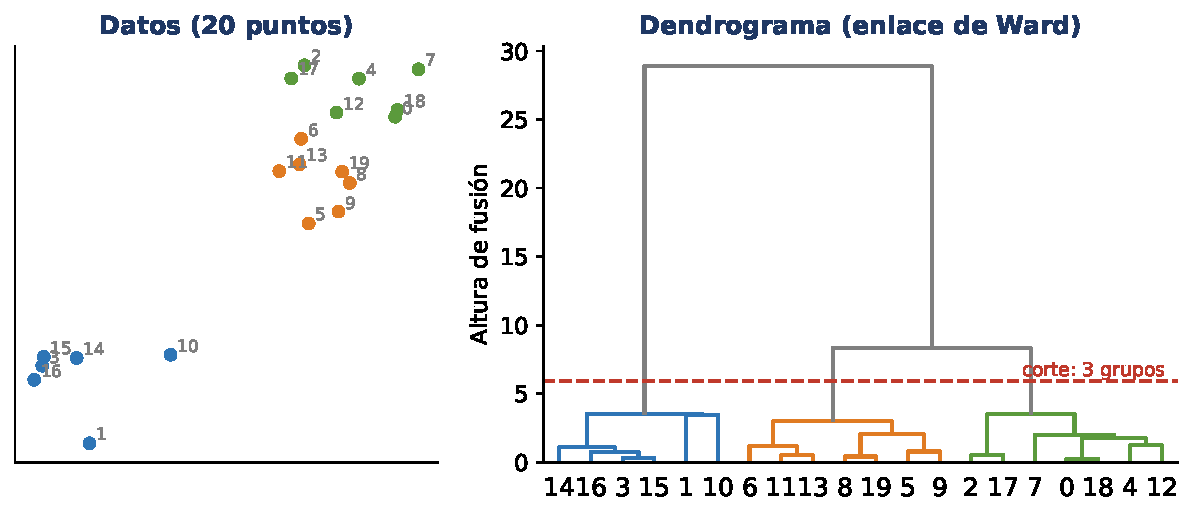
\includegraphics[width=0.72\textwidth]{dendrograma_corte}
  \small
  \begin{itemize}
    \item Cada hoja es un punto; cada unión horizontal es una fusión.
    \item La \textbf{altura} de una unión es la distancia entre los grupos que se fusionan.
    \item El orden horizontal de las hojas es arbitrario: dos hojas vecinas no necesariamente son cercanas.
          Lo que importa es la altura a la que se unen.
  \end{itemize}
\end{frame}

\begin{frame}{Distancia cofenética}
  \begin{itemize}
    \item La \textbf{distancia cofenética} $c_{ij}$ es la altura a la que $\x_i$ y $\x_j$ quedan
          por primera vez en el mismo grupo.
    \item En un dendrograma monótono es una \emph{ultramétrica}:
          $c_{ik} \le \max\{c_{ij},\, c_{jk}\}$.
    \item \textbf{Correlación cofenética}: correlación de Pearson entre las distancias originales
          $d_{ij}$ y las cofenéticas $c_{ij}$ de todos los pares.
  \end{itemize}
  \vspace{6pt}
  \begin{block}{Para qué sirve}
    Mide qué tan bien el árbol conserva las distancias originales: un valor cercano a 1
    indica que el dendrograma es un buen resumen de los datos. Permite comparar criterios
    de enlace sobre el mismo conjunto.
  \end{block}
\end{frame}

\begin{frame}{Cortar el árbol}
  \begin{itemize}
    \item \textbf{Por número de grupos}: cortar donde queden exactamente $k$ ramas
          (\texttt{criterion="maxclust"}).
    \item \textbf{Por altura}: cortar a una distancia $h$; quedan los grupos que se formaron
          por debajo de $h$ (\texttt{criterion="distance"}).
    \item \textbf{Por saltos}: un salto grande entre alturas de fusiones consecutivas indica que
          se están uniendo grupos muy distintos; cortar justo antes.
  \end{itemize}
  \vspace{6pt}
  \begin{block}{Una sola construcción, muchas particiones}
    El árbol se calcula una vez; cortarlo a distintas alturas no requiere recalcular.
    Se pueden comparar soluciones con distintos $k$ y validarlas con el método de silueta (Sesión 2)
    y con los índices de la Sesión 6.
  \end{block}
\end{frame}

% =====================================================================
\section{Complejidad y escalabilidad}
% =====================================================================

\begin{frame}{Complejidad computacional}
  \renewcommand{\arraystretch}{1.3}
  \begin{tabular}{@{}>{\raggedright\arraybackslash}p{0.38\textwidth}>{\raggedright\arraybackslash}p{0.25\textwidth}>{\raggedright\arraybackslash}p{0.27\textwidth}@{}}
    \toprule
    \textbf{Algoritmo} & \textbf{Tiempo} & \textbf{Memoria}\\
    \midrule
    Ingenuo (buscar el par más cercano en cada paso) & $O(n^3)$ & $O(n^2)$ \\
    Con colas de prioridad & $O(n^2\log n)$ & $O(n^2)$ \\
    Simple (árbol de expansión mínima, SLINK) & $O(n^2)$ & $O(n)$ \\
    Completo, promedio y Ward (cadena de vecinos más cercanos) & $O(n^2)$ & $O(n^2)$ \\
    \midrule
    k-medias (Sesión 2), por iteración & $O(nkd)$ & $O(nd)$ \\
    \bottomrule
  \end{tabular}
  \vspace{6pt}
  {\small SciPy usa los algoritmos de orden $O(n^2)$, pero primero calcula la matriz de distancias
  completa: la memoria limita antes que el tiempo.}
\end{frame}

\begin{frame}{¿Hasta dónde escala?}
  \centering
  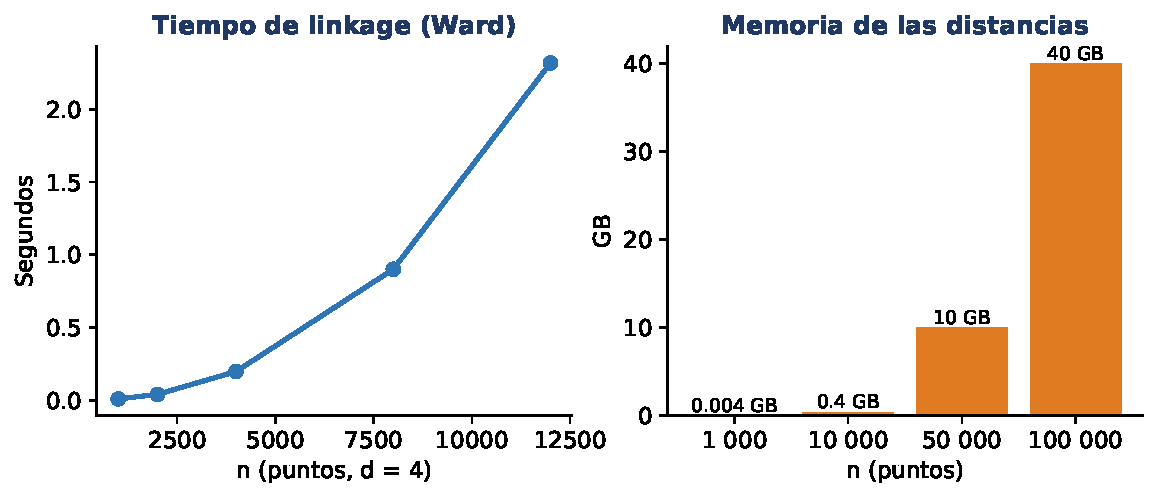
\includegraphics[width=0.82\textwidth]{escalabilidad}
  \begin{itemize}
    \item Izquierda: tiempo medido en una computadora de escritorio; crece cerca de $n^2$.
    \item Derecha: la matriz de distancias guarda $n(n-1)/2$ números de 8 bytes:
          con $n=100\,000$ ocupa 40 GB.
  \end{itemize}
\end{frame}

\begin{frame}{Estrategias para datos grandes}
  \begin{itemize}
    \item \textbf{Restricciones de conectividad}: sólo permitir fusiones entre vecinos
          (un grafo de $k$ vecinos), con \texttt{AgglomerativeClustering(connectivity=...)}.
    \item \textbf{Agrupar en dos etapas}: k-medias con muchos grupos pequeños (por ejemplo, 500)
          y después agrupamiento jerárquico de sus centros.
    \item \textbf{BIRCH}: resume los datos en un árbol de características en una sola pasada.
    \item \textbf{Muestreo}: construir el árbol con una muestra y asignar el resto al grupo más cercano.
  \end{itemize}
  \vspace{6pt}
  \begin{block}{Jerárquico frente a k-medias}
    \renewcommand{\arraystretch}{1.2}
    \begin{tabular}{@{}lll@{}}
      & \textbf{Jerárquico} & \textbf{k-medias}\\
      \midrule
      Fijar $k$ & no (se corta al final) & sí \\
      Resultado & determinista & depende de la inicialización \\
      Forma de los grupos & según el enlace & esféricos \\
      Escala a $n$ grande & hasta decenas de miles & millones \\
    \end{tabular}
  \end{block}
\end{frame}

\begin{frame}[fragile]{Agrupamiento jerárquico en SciPy y scikit-learn}
\begin{lstlisting}
from scipy.cluster.hierarchy import linkage, dendrogram, fcluster, cophenet
from scipy.spatial.distance import pdist

Z = linkage(X, method="ward")             # "single", "complete", "average", "ward"
# Cada fila de Z: [grupo i, grupo j, altura de la fusion, puntos en el nuevo grupo]
dendrogram(Z, truncate_mode="lastp", p=30) # dibujar las ultimas 30 fusiones
etiquetas = fcluster(Z, t=3, criterion="maxclust")   # cortar en 3 grupos
etiquetas = fcluster(Z, t=10, criterion="distance")  # cortar a la altura 10
c, _ = cophenet(Z, pdist(X))               # correlacion cofenetica

from sklearn.cluster import AgglomerativeClustering
ag = AgglomerativeClustering(n_clusters=3, linkage="ward").fit(X)
ag.labels_                                 # mismas etiquetas, sin dibujar el arbol
\end{lstlisting}
\end{frame}

% =====================================================================
%  Laboratorio (para omitirlo de las láminas, comentar la línea siguiente)
% =====================================================================
%  Laboratorio de la Sesión 3: agrupamiento jerárquico de Iris con SciPy
%  Se incluye desde Sesion3-Jerarquico.tex con % =====================================================================
%  Laboratorio de la Sesión 3: agrupamiento jerárquico de Iris con SciPy
%  Se incluye desde Sesion3-Jerarquico.tex con % =====================================================================
%  Laboratorio de la Sesión 3: agrupamiento jerárquico de Iris con SciPy
%  Se incluye desde Sesion3-Jerarquico.tex con \input{Laboratorio}
%  El mismo código, ejecutado, está en laboratorio_jerarquico.ipynb
% =====================================================================
\section{Laboratorio: agrupamiento jerárquico de Iris}
% =====================================================================

\begin{frame}[fragile]{Paso 1: construir el árbol}
\begin{lstlisting}
import numpy as np, pandas as pd
from sklearn.datasets import load_iris
from scipy.cluster.hierarchy import linkage, dendrogram, fcluster, cophenet
from scipy.spatial.distance import pdist

iris = load_iris()
X, especie = iris.data, iris.target   # medidas en cm; la especie NO se usa para agrupar

Z = linkage(X, method="ward")         # 149 fusiones
dendrogram(Z, no_labels=True)
\end{lstlisting}
  \begin{itemize}
    \item Como en la Sesión 2, se usan las medidas en centímetros sin estandarizar:
          todas tienen la misma unidad y los pétalos son las más informativas.
    \item \texttt{Z} tiene una fila por fusión: los dos grupos unidos, la altura y el tamaño del nuevo grupo.
    \item El dendrograma completo es el de la lámina del problema detonador.
  \end{itemize}
\end{frame}

\begin{frame}[fragile]{Paso 2: dónde cortar}
\begin{lstlisting}
print(Z[-6:, 2].round(2))   # alturas de las 6 ultimas fusiones
\end{lstlisting}
  \begin{columns}[c]
    \column{0.5\textwidth}
    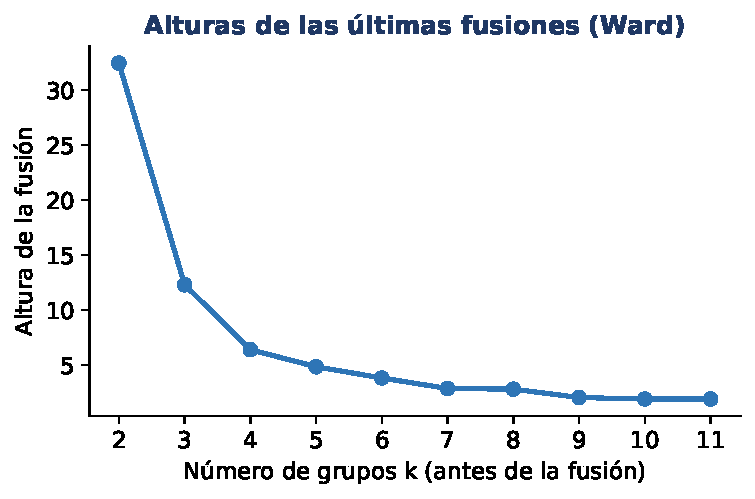
\includegraphics[width=\textwidth]{iris_alturas}
    \column{0.47\textwidth}
    \small
    Alturas de las últimas fusiones:
    2.87, 3.83, 4.85, 6.40, 12.30, 32.45.
    \begin{itemize}
      \item El salto más grande (de 12.3 a 32.5) está en la última fusión: el corte más claro deja \textbf{2 grupos}.
      \item El siguiente salto (de 6.4 a 12.3) sugiere \textbf{3 grupos}.
      \item Las dos escalas de Iris aparecen en un solo árbol: es la ambigüedad entre $k=2$ y $k=3$ de la Sesión 2.
    \end{itemize}
  \end{columns}
\end{frame}

\begin{frame}[fragile]{Paso 3: comparar los criterios de enlace}
\begin{lstlisting}
from sklearn.metrics import adjusted_rand_score
for metodo in ["single", "complete", "average", "ward"]:
    Z_m = linkage(X, method=metodo)
    c, _ = cophenet(Z_m, pdist(X))
    z = fcluster(Z_m, t=3, criterion="maxclust")
    print(metodo, round(c, 3), round(adjusted_rand_score(especie, z), 3), np.bincount(z)[1:])
\end{lstlisting}
  \begin{columns}[c]
    \column{0.42\textwidth}
    \small
    \begin{tabular}{@{}lccc@{}}
      \toprule
      \textbf{Enlace} & \textbf{Cofen.} & \textbf{ARI} & \textbf{Tamaños}\\
      \midrule
      Simple   & 0.86 & 0.56 & 98, 50, 2 \\
      Completo & 0.73 & 0.64 & 72, 50, 28 \\
      Promedio & 0.88 & 0.76 & 64, 50, 36 \\
      Ward     & 0.87 & 0.73 & 64, 50, 36 \\
      \bottomrule
    \end{tabular}\\[4pt]
    {\scriptsize Cofen.: correlación cofenética. ARI: índice de Rand ajustado contra la especie (Sesión 6), con $k=3$.}
    \column{0.56\textwidth}
    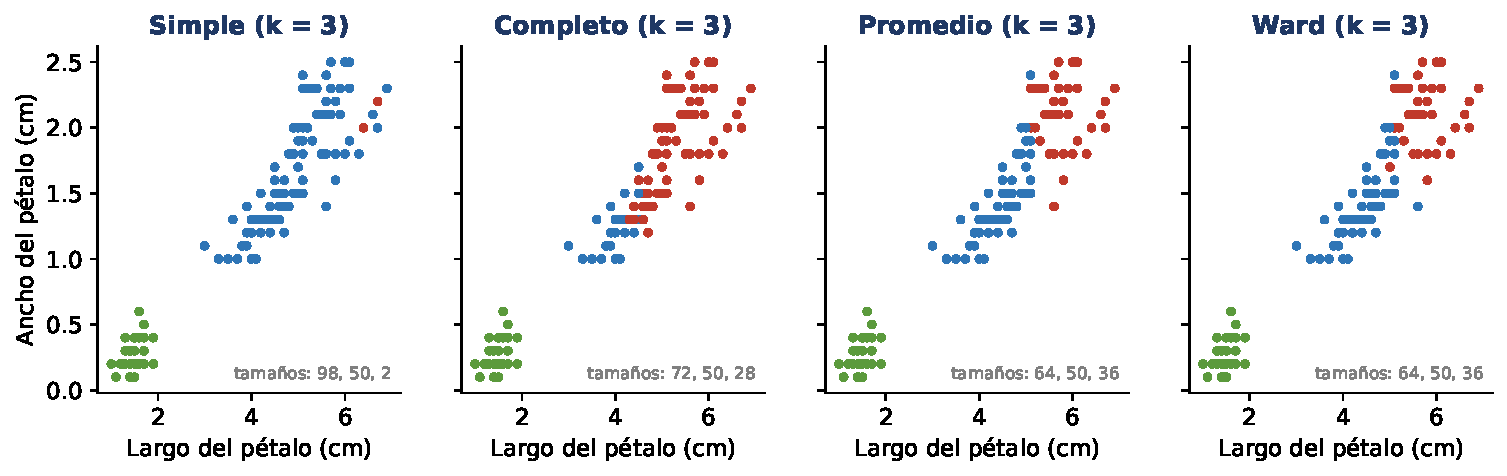
\includegraphics[width=\textwidth]{iris_enlaces}
  \end{columns}
\end{frame}

\begin{frame}{Paso 3: qué muestran los enlaces}
  \begin{itemize}
    \item \textbf{Simple}: separa setosa, pero con $k=3$ el tercer grupo tiene sólo 2 flores.
          Versicolor y virginica quedan encadenadas en un grupo de 98.
    \item \textbf{Completo}: con $k=2$ junta a setosa con 27 versicolor; con $k=3$ la aísla,
          pero parte versicolor en dos (23 y 27). Su correlación cofenética es la más baja (0.73).
    \item \textbf{Promedio} y \textbf{Ward}: tres grupos de 50, 64 y 36 flores, los más
          parecidos a las especies.
    \item El enlace promedio tiene la mayor correlación cofenética (0.88) y la mayor
          coincidencia con las especies (0.76).
  \end{itemize}
  \vspace{6pt}
  \begin{alertblock}{Lección}
    El criterio de enlace cambia el resultado tanto como el algoritmo. La correlación
    cofenética permite compararlos sin usar etiquetas.
  \end{alertblock}
\end{frame}

\begin{frame}{Paso 4: leer el dendrograma}
  \centering
  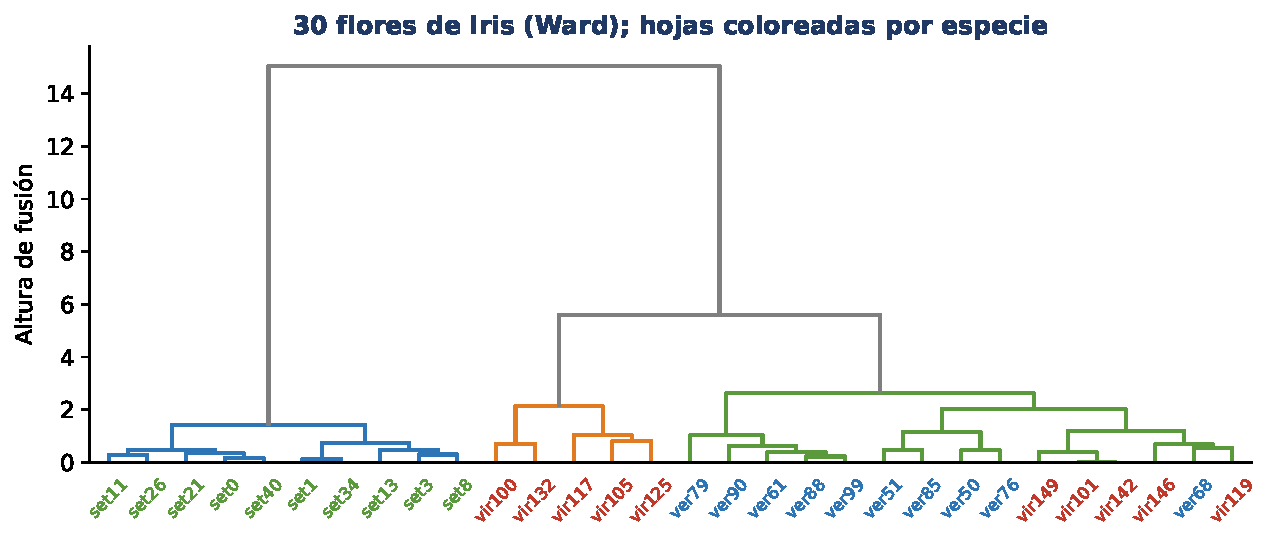
\includegraphics[width=0.72\textwidth]{iris_dendrograma_30}
  \small
  \begin{itemize}
    \item 30 flores, 10 por especie (la especie sólo colorea las hojas). Con 2 grupos: las
          10 setosas, y las 10 versicolor junto con las 10 virginica.
    \item Con 3 grupos: las setosas; 5 virginica; y las 10 versicolor con las otras 5 virginica.
    \item Las virginica que quedan con versicolor son las de pétalos más cortos
          (5.1 cm en promedio, contra 6.2 cm de las otras): se parecen más a versicolor.
  \end{itemize}
\end{frame}

\begin{frame}[fragile]{Paso 5: comparar con k-medias}
\begin{lstlisting}
from sklearn.cluster import KMeans
z_ward = fcluster(linkage(X, "ward"), t=3, criterion="maxclust")
z_km = KMeans(n_clusters=3, n_init=10, random_state=0).fit_predict(X)
print(pd.crosstab(z_ward, z_km))
print(adjusted_rand_score(z_ward, z_km))
\end{lstlisting}
  \begin{columns}[T]
    \column{0.48\textwidth}
    \small
    \begin{block}{Ward contra k-medias ($k=3$)}
      \begin{itemize}
        \item Coinciden en 148 de las 150 flores.
        \item Índice de Rand ajustado entre ambas particiones: 0.96.
        \item Contra la especie: 0.73 los dos.
      \end{itemize}
    \end{block}
    \column{0.48\textwidth}
    \small
    \begin{block}{Ward ($k=3$) contra la especie}
      \centering
      \begin{tabular}{@{}lccc@{}}
        & \textbf{setosa} & \textbf{versic.} & \textbf{virgin.}\\
        \midrule
        Grupo 1 & 50 & 0 & 0 \\
        Grupo 2 & 0 & 1 & 35 \\
        Grupo 3 & 0 & 49 & 15 \\
      \end{tabular}
    \end{block}
  \end{columns}
  \vspace{4pt}
  {\small Ward y k-medias optimizan el mismo criterio (la inercia): Ward lo hace de forma voraz,
  k-medias por iteraciones. Aquí llegan casi a la misma partición.}
\end{frame}

\begin{frame}{Conclusiones del laboratorio}
  \begin{itemize}
    \item Un solo dendrograma muestra las dos escalas de Iris: setosa contra el resto, y después
          versicolor contra virginica.
    \item Los saltos en las alturas de fusión orientan la elección de $k$ sin recalcular nada.
    \item El enlace importa: simple encadena, completo resume mal las distancias, y promedio y Ward
          dan los grupos más útiles.
    \item Ward reproduce casi exactamente el resultado de k-medias, sin depender de una inicialización.
    \item Ningún método separa por completo versicolor y virginica: sus medidas se traslapan.
  \end{itemize}
\end{frame}

%  El mismo código, ejecutado, está en laboratorio_jerarquico.ipynb
% =====================================================================
\section{Laboratorio: agrupamiento jerárquico de Iris}
% =====================================================================

\begin{frame}[fragile]{Paso 1: construir el árbol}
\begin{lstlisting}
import numpy as np, pandas as pd
from sklearn.datasets import load_iris
from scipy.cluster.hierarchy import linkage, dendrogram, fcluster, cophenet
from scipy.spatial.distance import pdist

iris = load_iris()
X, especie = iris.data, iris.target   # medidas en cm; la especie NO se usa para agrupar

Z = linkage(X, method="ward")         # 149 fusiones
dendrogram(Z, no_labels=True)
\end{lstlisting}
  \begin{itemize}
    \item Como en la Sesión 2, se usan las medidas en centímetros sin estandarizar:
          todas tienen la misma unidad y los pétalos son las más informativas.
    \item \texttt{Z} tiene una fila por fusión: los dos grupos unidos, la altura y el tamaño del nuevo grupo.
    \item El dendrograma completo es el de la lámina del problema detonador.
  \end{itemize}
\end{frame}

\begin{frame}[fragile]{Paso 2: dónde cortar}
\begin{lstlisting}
print(Z[-6:, 2].round(2))   # alturas de las 6 ultimas fusiones
\end{lstlisting}
  \begin{columns}[c]
    \column{0.5\textwidth}
    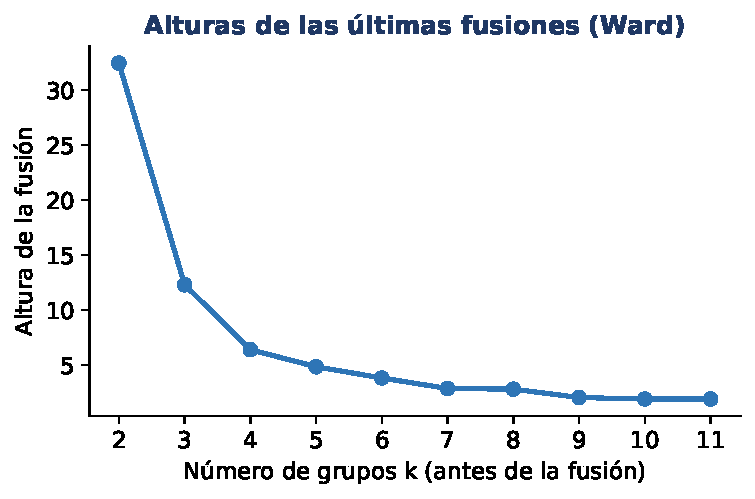
\includegraphics[width=\textwidth]{iris_alturas}
    \column{0.47\textwidth}
    \small
    Alturas de las últimas fusiones:
    2.87, 3.83, 4.85, 6.40, 12.30, 32.45.
    \begin{itemize}
      \item El salto más grande (de 12.3 a 32.5) está en la última fusión: el corte más claro deja \textbf{2 grupos}.
      \item El siguiente salto (de 6.4 a 12.3) sugiere \textbf{3 grupos}.
      \item Las dos escalas de Iris aparecen en un solo árbol: es la ambigüedad entre $k=2$ y $k=3$ de la Sesión 2.
    \end{itemize}
  \end{columns}
\end{frame}

\begin{frame}[fragile]{Paso 3: comparar los criterios de enlace}
\begin{lstlisting}
from sklearn.metrics import adjusted_rand_score
for metodo in ["single", "complete", "average", "ward"]:
    Z_m = linkage(X, method=metodo)
    c, _ = cophenet(Z_m, pdist(X))
    z = fcluster(Z_m, t=3, criterion="maxclust")
    print(metodo, round(c, 3), round(adjusted_rand_score(especie, z), 3), np.bincount(z)[1:])
\end{lstlisting}
  \begin{columns}[c]
    \column{0.42\textwidth}
    \small
    \begin{tabular}{@{}lccc@{}}
      \toprule
      \textbf{Enlace} & \textbf{Cofen.} & \textbf{ARI} & \textbf{Tamaños}\\
      \midrule
      Simple   & 0.86 & 0.56 & 98, 50, 2 \\
      Completo & 0.73 & 0.64 & 72, 50, 28 \\
      Promedio & 0.88 & 0.76 & 64, 50, 36 \\
      Ward     & 0.87 & 0.73 & 64, 50, 36 \\
      \bottomrule
    \end{tabular}\\[4pt]
    {\scriptsize Cofen.: correlación cofenética. ARI: índice de Rand ajustado contra la especie (Sesión 6), con $k=3$.}
    \column{0.56\textwidth}
    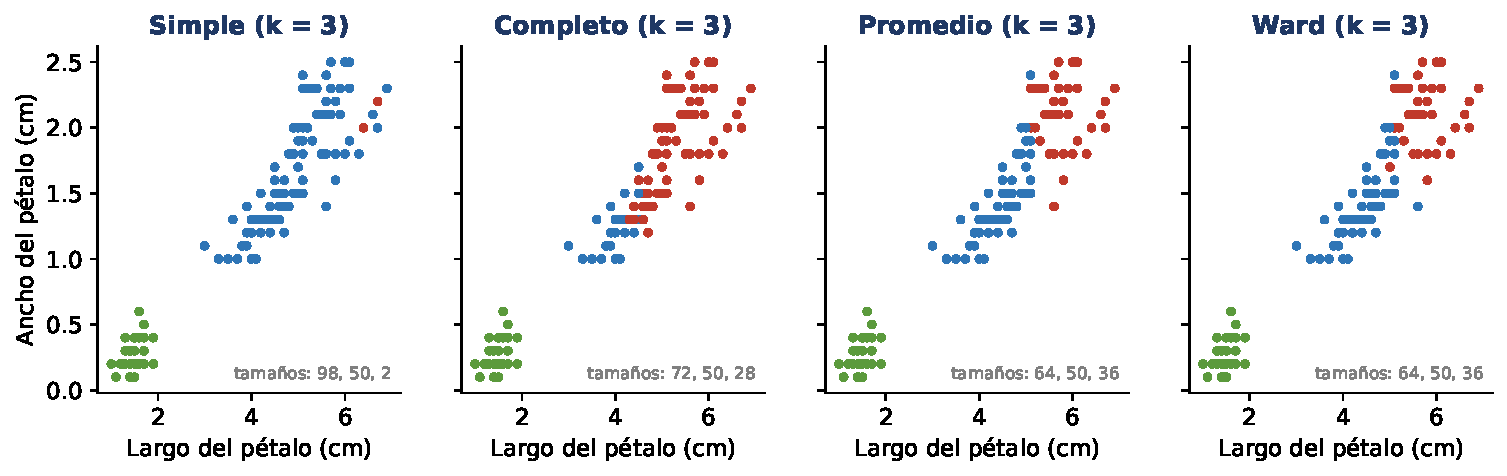
\includegraphics[width=\textwidth]{iris_enlaces}
  \end{columns}
\end{frame}

\begin{frame}{Paso 3: qué muestran los enlaces}
  \begin{itemize}
    \item \textbf{Simple}: separa setosa, pero con $k=3$ el tercer grupo tiene sólo 2 flores.
          Versicolor y virginica quedan encadenadas en un grupo de 98.
    \item \textbf{Completo}: con $k=2$ junta a setosa con 27 versicolor; con $k=3$ la aísla,
          pero parte versicolor en dos (23 y 27). Su correlación cofenética es la más baja (0.73).
    \item \textbf{Promedio} y \textbf{Ward}: tres grupos de 50, 64 y 36 flores, los más
          parecidos a las especies.
    \item El enlace promedio tiene la mayor correlación cofenética (0.88) y la mayor
          coincidencia con las especies (0.76).
  \end{itemize}
  \vspace{6pt}
  \begin{alertblock}{Lección}
    El criterio de enlace cambia el resultado tanto como el algoritmo. La correlación
    cofenética permite compararlos sin usar etiquetas.
  \end{alertblock}
\end{frame}

\begin{frame}{Paso 4: leer el dendrograma}
  \centering
  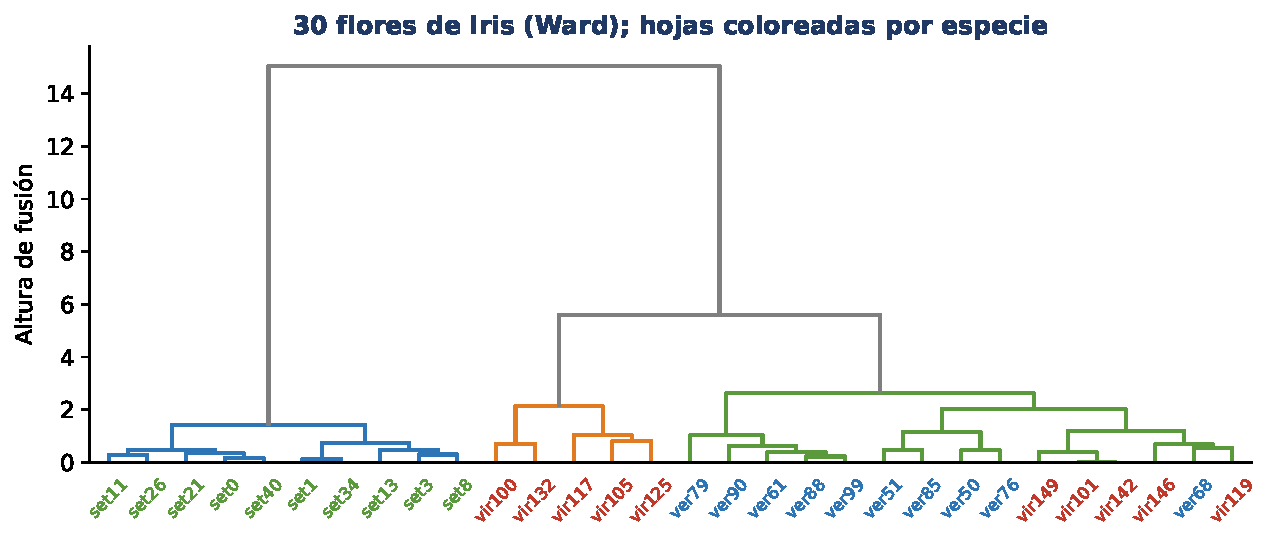
\includegraphics[width=0.72\textwidth]{iris_dendrograma_30}
  \small
  \begin{itemize}
    \item 30 flores, 10 por especie (la especie sólo colorea las hojas). Con 2 grupos: las
          10 setosas, y las 10 versicolor junto con las 10 virginica.
    \item Con 3 grupos: las setosas; 5 virginica; y las 10 versicolor con las otras 5 virginica.
    \item Las virginica que quedan con versicolor son las de pétalos más cortos
          (5.1 cm en promedio, contra 6.2 cm de las otras): se parecen más a versicolor.
  \end{itemize}
\end{frame}

\begin{frame}[fragile]{Paso 5: comparar con k-medias}
\begin{lstlisting}
from sklearn.cluster import KMeans
z_ward = fcluster(linkage(X, "ward"), t=3, criterion="maxclust")
z_km = KMeans(n_clusters=3, n_init=10, random_state=0).fit_predict(X)
print(pd.crosstab(z_ward, z_km))
print(adjusted_rand_score(z_ward, z_km))
\end{lstlisting}
  \begin{columns}[T]
    \column{0.48\textwidth}
    \small
    \begin{block}{Ward contra k-medias ($k=3$)}
      \begin{itemize}
        \item Coinciden en 148 de las 150 flores.
        \item Índice de Rand ajustado entre ambas particiones: 0.96.
        \item Contra la especie: 0.73 los dos.
      \end{itemize}
    \end{block}
    \column{0.48\textwidth}
    \small
    \begin{block}{Ward ($k=3$) contra la especie}
      \centering
      \begin{tabular}{@{}lccc@{}}
        & \textbf{setosa} & \textbf{versic.} & \textbf{virgin.}\\
        \midrule
        Grupo 1 & 50 & 0 & 0 \\
        Grupo 2 & 0 & 1 & 35 \\
        Grupo 3 & 0 & 49 & 15 \\
      \end{tabular}
    \end{block}
  \end{columns}
  \vspace{4pt}
  {\small Ward y k-medias optimizan el mismo criterio (la inercia): Ward lo hace de forma voraz,
  k-medias por iteraciones. Aquí llegan casi a la misma partición.}
\end{frame}

\begin{frame}{Conclusiones del laboratorio}
  \begin{itemize}
    \item Un solo dendrograma muestra las dos escalas de Iris: setosa contra el resto, y después
          versicolor contra virginica.
    \item Los saltos en las alturas de fusión orientan la elección de $k$ sin recalcular nada.
    \item El enlace importa: simple encadena, completo resume mal las distancias, y promedio y Ward
          dan los grupos más útiles.
    \item Ward reproduce casi exactamente el resultado de k-medias, sin depender de una inicialización.
    \item Ningún método separa por completo versicolor y virginica: sus medidas se traslapan.
  \end{itemize}
\end{frame}

%  El mismo código, ejecutado, está en laboratorio_jerarquico.ipynb
% =====================================================================
\section{Laboratorio: agrupamiento jerárquico de Iris}
% =====================================================================

\begin{frame}[fragile]{Paso 1: construir el árbol}
\begin{lstlisting}
import numpy as np, pandas as pd
from sklearn.datasets import load_iris
from scipy.cluster.hierarchy import linkage, dendrogram, fcluster, cophenet
from scipy.spatial.distance import pdist

iris = load_iris()
X, especie = iris.data, iris.target   # medidas en cm; la especie NO se usa para agrupar

Z = linkage(X, method="ward")         # 149 fusiones
dendrogram(Z, no_labels=True)
\end{lstlisting}
  \begin{itemize}
    \item Como en la Sesión 2, se usan las medidas en centímetros sin estandarizar:
          todas tienen la misma unidad y los pétalos son las más informativas.
    \item \texttt{Z} tiene una fila por fusión: los dos grupos unidos, la altura y el tamaño del nuevo grupo.
    \item El dendrograma completo es el de la lámina del problema detonador.
  \end{itemize}
\end{frame}

\begin{frame}[fragile]{Paso 2: dónde cortar}
\begin{lstlisting}
print(Z[-6:, 2].round(2))   # alturas de las 6 ultimas fusiones
\end{lstlisting}
  \begin{columns}[c]
    \column{0.5\textwidth}
    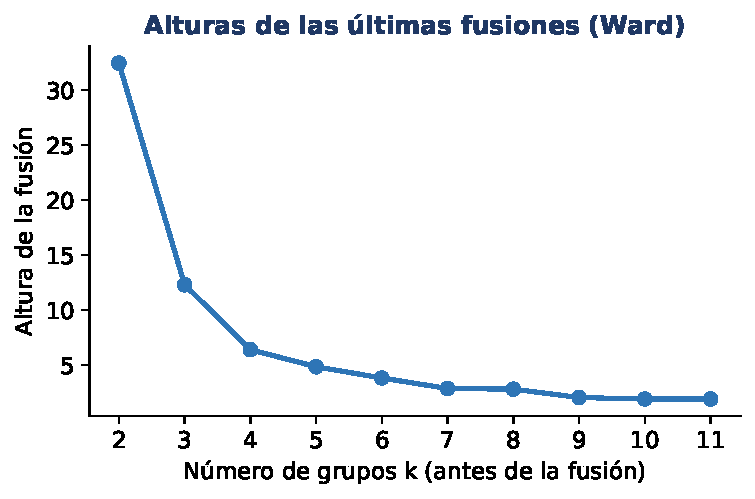
\includegraphics[width=\textwidth]{iris_alturas}
    \column{0.47\textwidth}
    \small
    Alturas de las últimas fusiones:
    2.87, 3.83, 4.85, 6.40, 12.30, 32.45.
    \begin{itemize}
      \item El salto más grande (de 12.3 a 32.5) está en la última fusión: el corte más claro deja \textbf{2 grupos}.
      \item El siguiente salto (de 6.4 a 12.3) sugiere \textbf{3 grupos}.
      \item Las dos escalas de Iris aparecen en un solo árbol: es la ambigüedad entre $k=2$ y $k=3$ de la Sesión 2.
    \end{itemize}
  \end{columns}
\end{frame}

\begin{frame}[fragile]{Paso 3: comparar los criterios de enlace}
\begin{lstlisting}
from sklearn.metrics import adjusted_rand_score
for metodo in ["single", "complete", "average", "ward"]:
    Z_m = linkage(X, method=metodo)
    c, _ = cophenet(Z_m, pdist(X))
    z = fcluster(Z_m, t=3, criterion="maxclust")
    print(metodo, round(c, 3), round(adjusted_rand_score(especie, z), 3), np.bincount(z)[1:])
\end{lstlisting}
  \begin{columns}[c]
    \column{0.42\textwidth}
    \small
    \begin{tabular}{@{}lccc@{}}
      \toprule
      \textbf{Enlace} & \textbf{Cofen.} & \textbf{ARI} & \textbf{Tamaños}\\
      \midrule
      Simple   & 0.86 & 0.56 & 98, 50, 2 \\
      Completo & 0.73 & 0.64 & 72, 50, 28 \\
      Promedio & 0.88 & 0.76 & 64, 50, 36 \\
      Ward     & 0.87 & 0.73 & 64, 50, 36 \\
      \bottomrule
    \end{tabular}\\[4pt]
    {\scriptsize Cofen.: correlación cofenética. ARI: índice de Rand ajustado contra la especie (Sesión 6), con $k=3$.}
    \column{0.56\textwidth}
    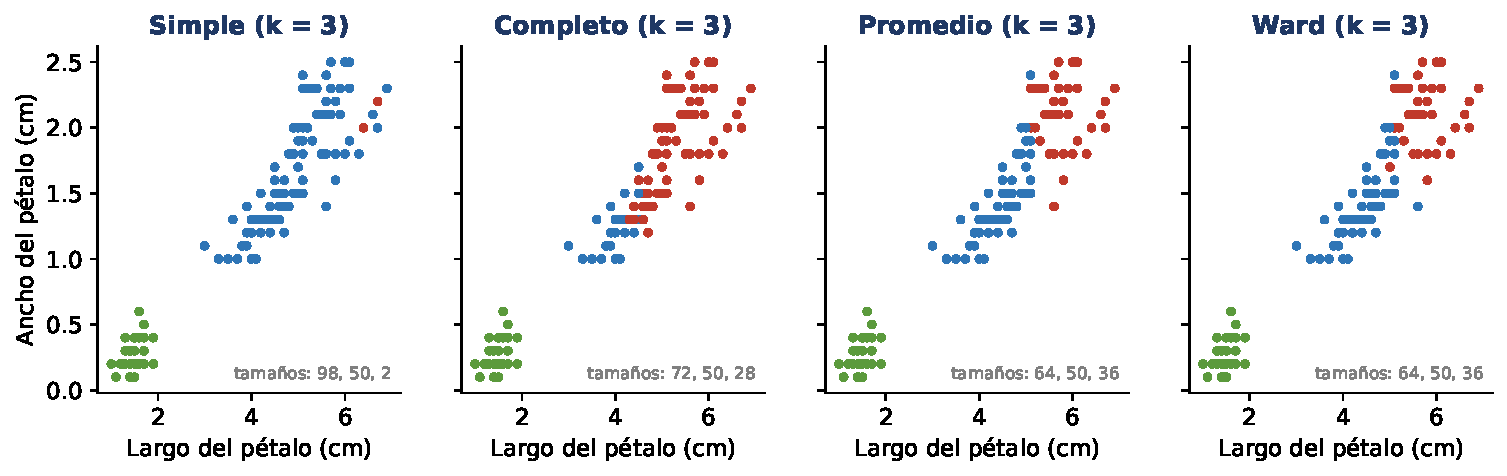
\includegraphics[width=\textwidth]{iris_enlaces}
  \end{columns}
\end{frame}

\begin{frame}{Paso 3: qué muestran los enlaces}
  \begin{itemize}
    \item \textbf{Simple}: separa setosa, pero con $k=3$ el tercer grupo tiene sólo 2 flores.
          Versicolor y virginica quedan encadenadas en un grupo de 98.
    \item \textbf{Completo}: con $k=2$ junta a setosa con 27 versicolor; con $k=3$ la aísla,
          pero parte versicolor en dos (23 y 27). Su correlación cofenética es la más baja (0.73).
    \item \textbf{Promedio} y \textbf{Ward}: tres grupos de 50, 64 y 36 flores, los más
          parecidos a las especies.
    \item El enlace promedio tiene la mayor correlación cofenética (0.88) y la mayor
          coincidencia con las especies (0.76).
  \end{itemize}
  \vspace{6pt}
  \begin{alertblock}{Lección}
    El criterio de enlace cambia el resultado tanto como el algoritmo. La correlación
    cofenética permite compararlos sin usar etiquetas.
  \end{alertblock}
\end{frame}

\begin{frame}{Paso 4: leer el dendrograma}
  \centering
  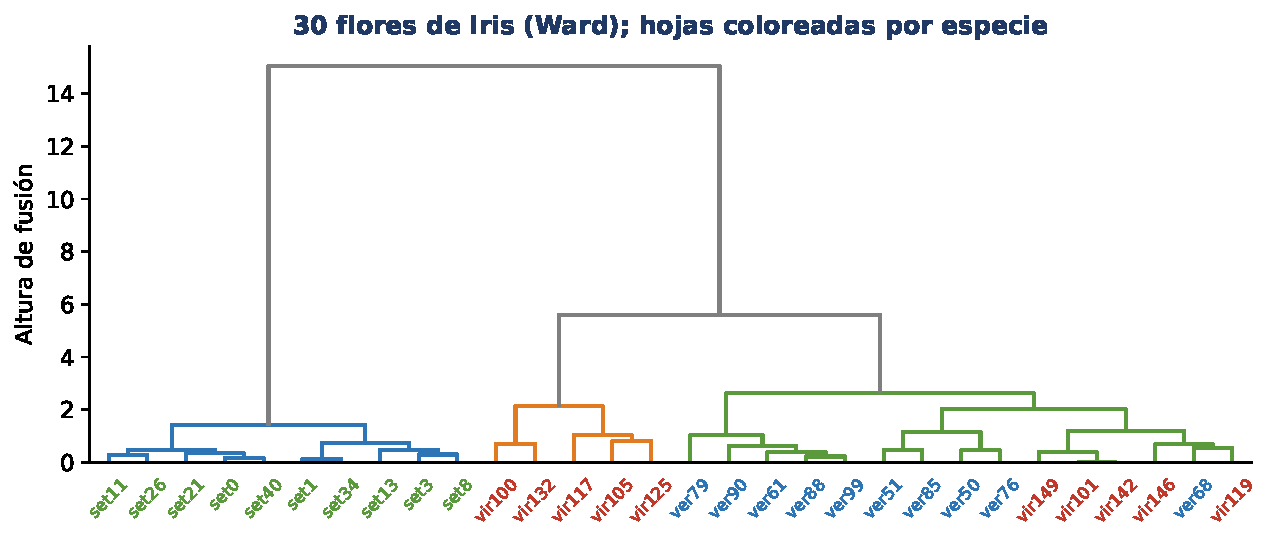
\includegraphics[width=0.72\textwidth]{iris_dendrograma_30}
  \small
  \begin{itemize}
    \item 30 flores, 10 por especie (la especie sólo colorea las hojas). Con 2 grupos: las
          10 setosas, y las 10 versicolor junto con las 10 virginica.
    \item Con 3 grupos: las setosas; 5 virginica; y las 10 versicolor con las otras 5 virginica.
    \item Las virginica que quedan con versicolor son las de pétalos más cortos
          (5.1 cm en promedio, contra 6.2 cm de las otras): se parecen más a versicolor.
  \end{itemize}
\end{frame}

\begin{frame}[fragile]{Paso 5: comparar con k-medias}
\begin{lstlisting}
from sklearn.cluster import KMeans
z_ward = fcluster(linkage(X, "ward"), t=3, criterion="maxclust")
z_km = KMeans(n_clusters=3, n_init=10, random_state=0).fit_predict(X)
print(pd.crosstab(z_ward, z_km))
print(adjusted_rand_score(z_ward, z_km))
\end{lstlisting}
  \begin{columns}[T]
    \column{0.48\textwidth}
    \small
    \begin{block}{Ward contra k-medias ($k=3$)}
      \begin{itemize}
        \item Coinciden en 148 de las 150 flores.
        \item Índice de Rand ajustado entre ambas particiones: 0.96.
        \item Contra la especie: 0.73 los dos.
      \end{itemize}
    \end{block}
    \column{0.48\textwidth}
    \small
    \begin{block}{Ward ($k=3$) contra la especie}
      \centering
      \begin{tabular}{@{}lccc@{}}
        & \textbf{setosa} & \textbf{versic.} & \textbf{virgin.}\\
        \midrule
        Grupo 1 & 50 & 0 & 0 \\
        Grupo 2 & 0 & 1 & 35 \\
        Grupo 3 & 0 & 49 & 15 \\
      \end{tabular}
    \end{block}
  \end{columns}
  \vspace{4pt}
  {\small Ward y k-medias optimizan el mismo criterio (la inercia): Ward lo hace de forma voraz,
  k-medias por iteraciones. Aquí llegan casi a la misma partición.}
\end{frame}

\begin{frame}{Conclusiones del laboratorio}
  \begin{itemize}
    \item Un solo dendrograma muestra las dos escalas de Iris: setosa contra el resto, y después
          versicolor contra virginica.
    \item Los saltos en las alturas de fusión orientan la elección de $k$ sin recalcular nada.
    \item El enlace importa: simple encadena, completo resume mal las distancias, y promedio y Ward
          dan los grupos más útiles.
    \item Ward reproduce casi exactamente el resultado de k-medias, sin depender de una inicialización.
    \item Ningún método separa por completo versicolor y virginica: sus medidas se traslapan.
  \end{itemize}
\end{frame}

% =====================================================================

\begin{frame}{Resumen}
  \begin{itemize}
    \item El agrupamiento jerárquico construye particiones anidadas; $k$ se elige al cortar el árbol.
    \item El aglomerativo une en cada paso los dos grupos más cercanos según el \textbf{criterio de enlace}.
    \item Simple sigue formas alargadas pero encadena; completo y Ward forman grupos compactos;
          Ward es la versión voraz de k-medias.
    \item El dendrograma se lee por alturas; la correlación cofenética mide qué tan bien resume los datos.
    \item Memoria $O(n^2)$: útil hasta decenas de miles de puntos.
  \end{itemize}
  \vspace{6pt}
  \begin{block}{Próxima sesión}
    Modelos de mezclas gaussianas: grupos elípticos y asignaciones con incertidumbre.
  \end{block}
\end{frame}

\end{document}
